\chapter{Μεθοδολογία}
\label{ch:methodology}

Σε αυτή την εργασία κάνουμε την υπόθεση ότι τα αντικείμενα του 
τρισδιάστατου χώρου αναπαρίστανται από την εξωτερική τους επιφάνεια 
η οποία περιγράφεται από τριγωνικά πλέγματα. 
Αυτή η υπόθεση δεν είναι περιοριστική, καθώς η προσαρμογή της μεθοδολογίας 
που ακολουθούμε σε περιγραφές άλλου τύπου δεν είναι δύσκολη.
Για την εφαρμογή της μεθοδολογίας θα πρέπει:
\begin{enumerate}
    \item Είτε οι αναπαραστάσεις διαφορετικού τύπου να μετατραπούν σε αναπαράσταση 
    με τριγωνικό πλέγμα (αυτή η μετατροπή είναι πάντοτε εφικτή, για παράδειγμα, 
    από πολυγωνικά πλέγματα).
    \item Είτε να δοθούν δύο ρουτίνες για τα στοιχεία από τα οποία αποτελείται η 
    αναπαράσταση. Η μία να υπολογίζει το \tl{AABB} του στοιχείου 
    ενώ η άλλη να υπολογίζει την Ευκλείδεια απόσταση δύο τέτοιων στοιχείων.
\end{enumerate}
Επιπλέον, σημειώνουμε ότι η χρήση επιφανειακών αναπαραστάσεων για τα αντικείμενα 
υπονοεί πως δε θα γίνει ανίχνευση σύγκρουσης εάν το ένα αντικείμενο περικλείει 
εντελώς το άλλο, αλλά τέτοιες καταστάσεις αποφεύγονται σε πολλές εφαρμογές.


\section{Στοιχειώδεις Γεωμετρικές Πράξεις}
\subsection{Ευκλείδεια Απόσταση δύο Τριγώνων}
\label{subsec:tria_distance}
% Έστω τα τρίγωνα $P$ και $Q$ στον $\mathbb{R}^3$.
% Η Ευκλείδεια απόσταση $d(P,Q)$ μεταξύ των τριγώνων $P$ και $Q$
% ορίζεται ως:
% \[ d(P,Q) = \min_{p \in P, q \in Q} |p - q| \]
% όπου με $|p-q|$ συμβολίζεται η Ευκλείδεια απόσταση των σημείων 
% $p$ και $q$.

% Έστω p,q

\subsubsection{Ευκλείδεια Απόσταση δύο Ευθυγράμμων Τμημάτων}
\subsubsection{Ευκλείδεια Απόσταση Σημείου και Τριγώνου}

\subsection{Γεωμετρικές Πράξεις για \tl{AABB}}
Ένα οριοθετικό πλαίσιο ευθυγραμμισμένο με τους άξονες (\tl{AABB})
είναι, απλώς, ένα ορθογώνιο παραλληλεπίπεδο του οποίου οι 
έδρες είναι κάθετες σε ένα από τα διανύσματα βάσης.

Ένα \tl{AABB} αναπαριστάται στη μνήμη από τα άκρα της κύριας 
διαγωνίου του.
Δηλαδή το σημείο $S$ με τις μικρότερες $x$, $y$, $z$ συντεταγμένες
και το σημείο $T$ με τις μεγαλύτερες $x$, $y$, $z$ συντεταγμένες.

\begin{figure}[h]
    \centering
    
    \newcommand{\Depth}{2}
    \newcommand{\Height}{2}
    \newcommand{\Width}{3}
    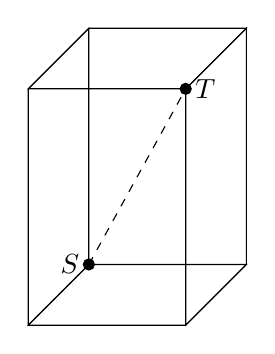
\begin{tikzpicture}
        \coordinate (O) at (0,0,0);
        \coordinate (A) at (0,\Width,0);
        \coordinate (B) at (0,\Width,\Height);
        \coordinate (C) at (0,0,\Height);
        \coordinate (D) at (\Depth,0,0);
        \coordinate (E) at (\Depth,\Width,0);
        \coordinate (F) at (\Depth,\Width,\Height);
        \coordinate (G) at (\Depth,0,\Height);

        \draw[] (O) -- (C) -- (G) -- (D) -- cycle;% Bottom Face
        \draw[] (O) -- (A) -- (E) -- (D) -- cycle;% Back Face
        \draw[] (O) -- (A) -- (B) -- (C) -- cycle;% Left Face
        \draw[] (D) -- (E) -- (F) -- (G) -- cycle;% Right Face
        \draw[] (C) -- (B) -- (F) -- (G) -- cycle;% Front Face
        \draw[] (A) -- (B) -- (F) -- (E) -- cycle;% Top Face

        \draw[fill=black] (O) circle (2pt) node[left]{$S$};
        \draw[fill=black] (F) circle (2pt) node[right]{$T$};
        \draw[dashed] (O) -- (F);
    \end{tikzpicture}
    \caption[Αναπαράσταση ενός \tl{AABB}]{Αναπαράσταση ενός \tl{AABB}}
\end{figure}

\subsubsection{Υπολογισμός Απόστασης \tl{AABB-AABB}}
Έστω τα ευθυγραμμισμένα με τους άξονες πλαίσια
$P$ και $Q$ στον $\mathbb{R}^3$.
Η Ευκλείδεια απόσταση $d(P,Q)$ μεταξύ των πλαισίων $P$ και $Q$
ορίζεται ως:
\[ d(P,Q) = \min_{p \in P, q \in Q} \lVert p - q \rVert \]
όπου με $\lVert p - q \rVert$ συμβολίζεται η Ευκλείδεια 
απόσταση των σημείων $p$ και $q$.

Για τον υπολογισμό της απόστασης μεταξύ δύο τέτοιων πλαισίων, 
εκμεταλλευόμαστε το γεγονός ότι οι πλευρές τους είναι ευθυγραμμισμένες
με του άξονες.
Έτσι μπορούμε να υπολογίσουμε την απόσταση χωρίζοντας τη στις συνιστώσες της.
Τελικά, προκύπτει ο αλγόριθμος \ref{alg:aabb_dist}, 
όμοιος με αυτόν που περιγράφεται στο \cite{krishnamurthy2011gpu}.
Στον παραπάνω αλγόριθμο  ο τελεστής "$-$" στις γραμμές 
$1$,$2$ είναι διανυσματική αφαίρεση των συντεταγμένων των σημείων.
Ο τελεστής \tl{\texttt{max(0, $v$)}} είναι επίσης διανυσματικός και
αντικαθιστά όλες τις αρνητικές τιμές ενός διανύσματος $v$
με $0$.
Ο τελεστής $\cdot$ είναι το εσωτερικό γινόμενο διανυσμάτων.

\selectlanguage{english}
\IncMargin{1.5em}
\begin{algorithm}[H]
    \label{alg:aabb_dist}
    \caption[Υπολογισμός Απόστασης δύο \tl{AABB}]{
        \tg{Υπολογισμός της Ευκλείδειας Απόστασης δύο AABB}
    }
    \DontPrintSemicolon
    \KwIn{Two AABBs $P$, $Q$}
    \KwOut{Euclidean distance of $P$ and $Q$}
    \SetKwFunction{funcname}{AABB\_distance}
    \SetKwFunction{max}{max}
    \Indm\nonl\funcname($P$, $Q$)\\
    \Indp
        $w \gets \max(0, P.S - Q.T)$\;
        $v \gets \max(0, Q.S - P.T)$\;
        \Return{$\sqrt{v \cdot v + w \cdot w}$}

    
\end{algorithm}
\DecMargin{1.5em}
\selectlanguage{greek}

\subsubsection{Κατασκευή \tl{AABB} Από Τρίγωνο}
Με τον αλγόριθμο \ref{alg:aabb_from_triangle} κατασκευάζουμε 
ένα \tl{AABB} που εξ' ολοκλήρου περικλείει ένα τρίγωνο.
Η ρουτίνα \tl{\texttt{vertices($T$)}} επιστρέφει τις 
τρεις κορυφές του τριγώνου $T$.
Οι τελεστές \tl{\texttt{min(), max()}} είναι διανυσματικοί,
δέχονται ως όρισμα μια λίστα από διανύσματα και επιστρέφουν 
ένα διάνυσμα με τις ελάχιστες/μέγιστες συντεταγμένες ανά άξονα.

\selectlanguage{english}
\IncMargin{1.5em}
\begin{algorithm}[H]
    \label{alg:aabb_from_triangle}
    \caption[Κατασκευή \tl{AABB} από Τρίγωνο]{
        \tg{Κατασκευή \tl{AABB} από Τρίγωνο}
        }
    \DontPrintSemicolon
    \KwIn{A triangle $T$}
    \KwOut{An AABB enclosing $T$}
    \SetKwFunction{funcname}{AABB}
    \SetKwFunction{min}{min}
    \SetKwFunction{max}{max}
    \SetKwFunction{vertices}{vertices}
    \Indm\nonl\funcname($T$)\\
    \Indp
        $S \gets \min(\vertices(T))$\;
        $T \gets \max(\vertices(T))$\; 
        \Return{ \{$S$, $T$\}}
    
\end{algorithm}
\DecMargin{1.5em}
\selectlanguage{greek}

\subsubsection{Συνένωση Δύο \tl{AABB}}
Ο αλγόριθμος \ref{alg:combine_aabbs} κατασκευάζει ένα \tl{AABB} περικλείει
εξ' ολοκλήρου δύο άλλα \tl{AABB} που δέχεται ως ορίσματα. 
Αυτή η πράξη είναι χρήσιμη γιατί αν έχουμε ήδη βρει τα \tl{AABB} για δύο 
ομάδες αντικειμένων ξεχωριστά, μπορούμε σε σταθερό χρόνο $\bigO(1)$ να 
κατασκευάσουμε το \tl{AABB} που περικλείει όλα τα αντικείμενα. 
Οι τελεστές \tl{\texttt{min(), max()}} είναι ίδιοι με πριν.

\selectlanguage{english}
\IncMargin{1.5em}
\begin{algorithm}[H]
    \label{alg:combine_aabbs}
    \caption[Κατασκευή \tl{AABB} από δύο άλλα \tl{AABB}]{
        \tg{Κατασκευή \tl{AABB} από δύο άλλα \tl{AABB}}
    }
    \DontPrintSemicolon
    \KwIn{Two AABBs $P$, $Q$}
    \KwOut{An AABB enclosing $P$ and $Q$}
    \SetKwFunction{combineAABB}{combine\_AABB}
    \Indm\nonl\combineAABB($P$, $Q$)\\
    \Indp
        
    $S \gets \min(P.S, Q.S)$\;
    $T \gets \max(P.T, Q.T)$\; 
    \Return{ \{$S$, $T$\}}
\end{algorithm}
\DecMargin{1.5em}
\selectlanguage{greek}

\section{Αλγόριθμοι Εξαντλητικής Αναζήτησης}
\label{sec:exhaustive_search}
Έστω δύο αντικείμενα του τρισδιάστατου χώρου που αναπαρίστανται από 
τριγωνικά πλέγματα.
Από τον ορισμό της Ευκλείδειας απόστασης δύο τριγωνικών πλεγμάτων που
δόθηκε στην ενότητα \ref{sec:problem_description} και τη χρήση μιας 
ρουτίνας \tl{\texttt{triangle\_distance(p, q)}}, προκύπτει ο 
τετριμμένος αλγόριθμος \ref{alg:exhaustive_search}. 
Η πολυπλοκότητα του αλγορίθμου είναι $\bigO(N*M)$, όπου 
$N$ και $M$ είναι το πλήθος των τριγώνων των δύο αντικειμένων.

\selectlanguage{english}
\IncMargin{1.5em}
\begin{algorithm}[h]
    \caption[Απόσταση Τριγωνικών Πλεγμάτων με Πλήρη Αναζήτηση]{
        \tg{Απόσταση Τριγωνικών Πλεγμάτων με Πλήρη Αναζήτηση}
        }
    \label{alg:exhaustive_search}
    \DontPrintSemicolon
    \KwIn{Two triangle meshes $P$, $Q$}
    \KwOut{Euclidean distance of $P$ and $Q$}
    \SetKwFunction{dist}{triangle\_distance}
    \SetKwFunction{trias}{triangles}
    \SetKwFunction{min}{min}
    \SetKwFunction{exhaustivesearch}{triangle\_mesh\_distance}
    \Indm\nonl\exhaustivesearch ($P$, $Q$)\\
    \Indp
        $T_P \gets$ \trias($P$) \;
        $T_Q \gets$ \trias($Q$) \; 
        $distance \gets \inf$ \;
        \ForEach{$p \in T_P$}{
            \ForEach{$q \in T_Q$}{
                $distance \gets \min(distance, \dist(p,q))$\;
            }
        }
        \Return{$distance$}
\end{algorithm}
\DecMargin{1.5em}
\selectlanguage{greek}

Σύμφωνα με τη μελέτη που έγινε στην ενότητα \ref{sec:bounding_volumes}
μπορούμε να επιταχύνουμε τον χρόνο εκτέλεσης του αλγορίθμου αν 
χρησιμοποιήσουμε οριοθετικούς όγκους.
Συγκεκριμένα, θα χρησιμοποιήσουμε Οριοθετικά Πλαίσια Ευθυγραμμισμένα 
με τους Άξονες (\tl{AABB}). 
Όπως φαίνεται από τον πίνακα της ενότητας \ref{sec:geom_tests_cost},
ο υπολογισμός της ελάχιστης απόστασης \textit{\tl{AABB - AABB}} είναι πολύ πιο 
"οικονομικός" υπολογιστικά σε σχέση με τον υπολογισμό της απόστασης 
\textit{τρίγωνο - τρίγωνο}.
Μπορούμε να εκμεταλλευτούμε αυτό το γεγονός και σε συνδυασμό με το παρακάτω λήμμα 
να σχεδιάσουμε έναν ταχύτερο αλγόριθμο.

\begin{lemma}
    Έστω δύο σύνολα $S_A$ και $S_B$ που αποτελούνται από χωρικά αντικείμενα. 
    Έστω οι οριοθετικοί όγκοι $BV_A$ και $BV_B$ που εξ' ολοκλήρου περικλείουν 
    τα αντικείμενα των σύνολων  $S_A$ και $S_B$, αντίστοιχα. Τότε:
    
    \[ distance(BV_A, BV_B) \leq distance(a, b) , 
    \forall a \in S_A, \forall b \in S_B \]

    Δηλαδή, η Ευκλείδεια απόσταση οποιουδήποτε ζεύγους αντικειμένων από τα δύο σύνολα 
    θα είναι μεγαλύτερη ή ίση με την Ευκλείδεια απόσταση των οριοθετικών όγκων 
    των συνόλων.
    \label{lemma:box_distance}
\end{lemma}


\begin{proof}
    Συμβολίζουμε με $BV_A$ το σύνολο των σημείων του 
    οριοθετικού όγκου, $BV_A$. 
    Όμοια και για το σύνολο $BV_B$.

    Επίσης, έχουμε
    $S_A = \bigcup\limits_{a \in S_A} a $ και $S_B = \bigcup\limits_{b \in S_B} b$,
    όπου με $a$, $b$ συμβολίζουμε το σύνολο των σημείων των 
    χωρικών αντικειμένων $a$ και $b$.

    Αφού οι οριοθετικοί όγκοι περικλείουν τα σύνολα των 
    αντικειμένων $S_A$ και $S_B$ ισχύει επίσης ότι 
    $S_A \subseteq BV_A $ και 
    $S_B \subseteq BV_B $.

    Έστω ότι υπάρχουν αντικείμενα $a \in S_A$, $b \in S_B$ με απόσταση μικρότερη 
    από αυτή των οριοθετικών όγκων. Τότε, υπάρχουν σημεία $p \in a \subseteq S_A 
    \subseteq BV_A$ και $q \in b \subseteq S_B \subseteq BV_A$ ώστε 
    \[\lVert p - q \rVert < distance(BV_A, BV_B)\]
    Από τον ορισμό της Ευκλείδειας απόστασης δύο οριοθετικών όγκων καταλήγουμε 
    σε άτοπο.
\end{proof}

Προκύπτει, λοιπόν, ο αλγόριθμος \ref{alg:exhaustive_search_aabb}.
Αρχικά, κάθε τρίγωνο περικλείεται από 
ένα \tl{AABB}. Σε κάθε βήμα του αλγορίθμου είναι γνωστή η μικρότερη απόσταση 
που έχει υπολογιστεί μέχρι εκείνη τη στιγμή. Έτσι, για κάθε ζεύγος τριγώνων, 
πρώτα γίνεται ο γρήγορος υπολογισμός απόστασης \tl{AABB-AABB} και μόνο όταν αυτή 
η απόσταση είναι μικρότερη από την τρέχουσα απόσταση γίνεται ο έλεγχος 
τρίγωνο-τρίγωνο.
Η υπολογιστική πολυπλοκότητα παραμένει $\bigO(N*M)$, όπως και πριν.
Σημειώνεται, ότι ο χρόνος εκτέλεσης επηρεάζεται από τη σειρά που θα γίνουν 
οι πράξεις. Δηλαδή αν η μικρότερη απόσταση βρεθεί από πολύ νωρίς, τότε 
θα γίνουν πολύ λίγοι υπολογισμοί τρίγωνο-τρίγωνο, ενώ το αντίθετο θα συμβεί 
αν η μικρότερη απόσταση βρεθεί πιο αργά.

\selectlanguage{english}
\IncMargin{1.5em}
\begin{algorithm}[h]
    \caption[Απόσταση Τριγωνικών Πλεγμάτων με Πλήρη Αναζήτηση και \tl{AABB}]{
        \tg{Απόσταση Τριγωνικών Πλεγμάτων με Πλήρη Αναζήτηση και} AABB
        }
    \label{alg:exhaustive_search_aabb}
    \DontPrintSemicolon
    \KwIn{Two triangle meshes $P$, $Q$}
    \KwOut{Euclidean distance of $P$ and $Q$}
    \SetKwFunction{dist}{triangle\_distance}
    \SetKwFunction{aabbdist}{AABB\_distance}
    \SetKwFunction{trias}{triangles}
    \SetKwFunction{min}{min}
    \SetKwFunction{aabb}{AABB}
    \SetKwFunction{funcname}{triangle\_mesh\_distance}
    \Indm\nonl\funcname($P$, $Q$)\\
    \Indp
        $T_P \gets$ \trias($P$) \;
        $T_Q \gets$ \trias($Q$) \;
        precalculate AABBs of $T_P$\;
        precalculate AABBs of $T_Q$\; 
        $distance \gets \inf$ \;
        \ForEach{$p \in T_P$}{
            \ForEach{$q \in T_Q$}{
                \If{\aabbdist(\aabb($p$), \aabb($q$)) $ < distance$}{
                    $distance \gets \min(distance, \dist(p,q))$\;
                }
            }
        }
        \Return{$distance$}
\end{algorithm}
\DecMargin{1.5em}
\selectlanguage{greek}

Παραπάνω, θα μπορούσαμε να χρησιμοποιήσουμε οποιονδήποτε τύπο οριοθετικού όγκου.
Οι λόγοι για τους οποίους γίνεται η επιλογή των \tl{AABB} είναι:
\begin{enumerate}
    \item Η Ιεραρχία Οριοθετικών Όγκων που σχεδιάζουμε και προτείνουμε 
    στην ενότητα \ref{sec:design_bvh} χρησιμοποιεί επίσης \tl{AABB}.
    Επομένως, μπορεί να υπάρξει ένα μέτρο σύγκρισης μεταξύ των 
    αλγορίθμων.
    \item Η κατασκευή ενός \tl{AABB} 
    που περικλείει εξ' ολοκλήρου ένα τρίγωνο και έχει ελάχιστο όγκο 
    είναι εύκολη (αλγόριθμος \ref{alg:aabb_from_triangle}).
    \item Ο υπολογισμός της Ευκλείδειας απόστασης 
    δύο \tl{AABB} (αλγόριθμος \ref{alg:aabb_dist}) είναι 
    εύκολος (αλγόριθμος \ref{alg:aabb_dist}).
    \item Η συνένωση δύο \tl{AABB} για την κατασκευή 
    ενός μεγαλύτερου που περικλείει και τα δύο είναι επίσης 
    εύκολη (αλγόριθμος \ref{alg:combine_aabbs}). 
    Η συνένωση είναι χρήσιμη πράξη για την κατασκευή της 
    ιεραρχίας. 
\end{enumerate}

\section{Ορισμός Μετρικής Κόστους Αναζήτησης}
\label{sec:cost_metric}

Σε αυτήν την ενότητα, ορίζουμε μια μετρική κόστους αναζήτησης
ώστε να μπορούμε να συγκρίνουμε την επίδοση των αλγορίθμων που μελετώνται.
Η ίδια μετρική χρησιμοποιείται και στα \cite{gottschalk1996obbtree},
\cite{larsen1999fast} για τη σύγκριση διάφορων ιεραρχικών δομών δεδομένων.
Δοθέντος δύο αντικειμένων, το συνολικό κόστος για τον υπολογισμό της μεταξύ τους 
Ευκλείδειας απόστασης μπορεί να δοθεί από την ακόλουθη εξίσωση κόστους:

\[ T = N_v \times C_v + N_p \times C_p \]

Όπου 
\begin{description}
    \item[$T$] το συνολικό κόστος για τον υπολογισμό της απόστασης,
    \item[$N_v$] το πλήθος των υπολογισμών απόστασης μεταξύ οριοθετικών όγκων,
    \item[$C_v$] το κόστος υπολογισμού απόστασης μεταξύ οριοθετικών όγκων,
    \item[$N_p$] το πλήθος των υπολογισμών απόστασης μεταξύ των \tl{primitives}
    \footnote{\tl{Geometric primitives} είναι κάποια απλά γεωμετρικά σχήματα 
    που μπορεί να χειριστεί ένα σύστημα. Συνήθως είναι σημεία, πολύγωνα, πολύεδρα κλπ.}
    \item[$C_p$] το κόστος υπολογισμού απόστασης μεταξύ των \tl{primitives}
\end{description}

Η επιλογή του τύπου οριοθετικού όγκου που θα χρησιμοποιηθεί, κατά τη σχεδίαση μιας 
ιεραρχίας, διέπεται από δύο αντικρουόμενους περιορισμούς\footnote{
    Στις ενότητες \ref{sec:bounding_volumes}, \ref{sec:bvh}, γίνεται 
    λεπτομερέστερη περιγραφή για αυτό το \tl{trade-off} 
}:
\begin{enumerate}
    \item Θα πρέπει να ακολουθεί το μοντέλο όσο πιο στενά γίνεται (\tl{tight-fit})
    για να μειωθούν οι τιμές $N_v$, $N_p$.
    \item Ο υπολογισμός της απόστασης μεταξύ οριοθετικών όγκων να είναι όσο το 
    δυνατόν ταχύτερος (για να μειωθεί το κόστος $C_v$)
\end{enumerate}

Για αυτή την εργασία οι οριοθετικοί όγκοι είναι \tl{AABB}, ενώ τα \tl{primitives} 
είναι τρίγωνα.
Τα κόστη $C_v$, $C_p$ δίνονται στους πίνακες της ενότητας \ref{sec:geom_tests_cost}.
Οι τιμές των $N_v$, $N_p$ μετρώνται πειραματικά ανάλογα με τα δεδομένα εισόδου 
(γεωμετρία, μέγεθος, προσανατολισμό, ποιότητα των πλεγμάτων).


Σημείωση: στην παραπάνω μετρική κόστους δεν προσμετράται το κόστος προεπεξεργασίας 
των δεδομένων (πχ για την κατασκευή μιας ιεραρχίας).
Το συνολικό κόστος (προ-επεξεργασία και αναζήτηση) "συμπεριλαμβάνεται" στη
μέτρηση των χρόνων εκτέλεσης των πειραμάτων.


\section{Σχεδιασμός μιας Δομής \tl{BVH}, το \tl{sKD-Tree}}
\label{sec:design_bvh}
Για τον υπολογισμό της απόστασης των δύο πλεγμάτων αποδοτικά, 
αρχικά κάνουμε μια προ-επεξεργασία των δεδομένων οργανώνοντας 
τα σε μια Ιεραρχία Οριοθετικών Όγκων (\tl{BVH}).
Έπειτα σχεδιάζουμε αλγορίθμους, που εκμεταλλευόμενοι αυτή την 
ιεραρχική οργάνωση, παρουσιάζουν καλύτερη υπολογιστική πολυπλοκότητα,
μέσης περίπτωσης, σε σχέση με τους αλγορίθμους εξαντλητικής αναζήτησης.
Επειδή ο τρόπος οργάνωσης των χωρικών δεδομένων είναι παρόμοιος  
με τον τρόπο κατασκευής του \tl{KD-Tree}, η δομή που προτείνουμε 
ονομάζεται \tl{spatial KD-Tree} ή \tl{sKD-Tree}.

\subsection{Κατασκευή του \tl{sKD-Tree}}
Το \tl{sKD-Tree} είναι ένα σχεδόν πλήρες, ισορροπημένο, δυαδικό δέντρο
που χρησιμοποιεί \tl{AABB} για την οργάνωση των αντικειμένων. 
Η ιεραρχία κατασκευάζεται με βάση τα στοιχεία (\tl{elements/primitives})
ενός αντικειμένου.
Στην περίπτωση μας τα στοιχεία είναι τρίγωνα.
Κάθε κόμβος του δέντρου είναι ένα \tl{AABB}, ενώ το δέντρο έχει τις 
παρακάτω ιδιότητες:
\begin{itemize}
    \item Η ένωση των AABB των φύλλων του δέντρου περικλείει εξ' 
    ολοκλήρου την επιφάνεια του αντικειμένου.
    \item Το \tl{AABB} ενός κόμβου περικλείει εξ' ολοκλήρου τα 
    \tl{AABB} όλων των απογόνων του. 
\end{itemize}

Η ιδέα για την κατασκευή της ιεραρχίας είναι η ακόλουθη:
Αρχικά, τα φύλλα του δέντρου σχεδόν προσεγγίζουν την επιφάνεια του αντικειμένου και
οι εσωτερικοί κόμβοι αναπαριστούν προσεγγίσεις των απογόνων φύλλων τους.
Έτσι, όσο πιο κοντά στη ρίζα βρίσκεται ένας κόμβος, τόσο πιο αδρή είναι η 
προσέγγιση της επιφάνειας.
Η οργάνωση αυτή είναι χρήσιμη, γιατί με βάση το \tl{AABB} κάποιου εσωτερικού 
κόμβου, μπορεί να βρεθεί το κάτω φράγμα της απόστασης προς οποιοδήποτε στοιχείο
της επιφάνειας.

Το πρώτο βήμα για την κατασκευή του \tl{sKD-Tree} είναι η επικάλυψη 
των τριγώνων του πλέγματος με \tl{AABB}.
Αυτά θα αποτελούν τα φύλλα του δέντρου.
Έπειτα ακολουθούμε μια στρατηγική από πάνω προς τα κάτω ξεκινώντας 
από τη ρίζα του δέντρου. 
Σε κάθε βήμα, τα $n$ τρίγωνα του κόμβου χωρίζονται σε δύο υποσύνολα 
μεγέθους $\lfloor n/2\rfloor$ και $\lceil n/2 \rceil$ αντίστοιχα.
Για κάθε ένα από τα σύνολα, καλείται η αναδρομική ρουτίνα που δημιουργεί 
τα δύο υποδέντρα.  
Στη συνέχεια, τα \tl{AABB} των δύο παιδιών του κόμβου ενώνονται 
και δημιουργείται το \tl{AABB} του τρέχοντος κόμβου.
Η αναδρομή σταματά όταν το σύνολο αποτελείται από ένα μόνο τρίγωνο, 
του οποίου το \tl{AABB} είχαμε υπολογίσει στην αρχή.

Για τον διαχωρισμό των τριγώνων σε δύο υποσύνολα, αρχικά, επιλέγεται 
ένα \textit{αντιπροσωπευτικό σημείο} για κάθε τρίγωνο.
Στην υλοποίηση μας, το αντιπροσωπευτικό σημείο για το κάθε τρίγωνο 
επιλέγεται να είναι το κέντρου του \tl{AABB} του\footnote{Επιλέγουμε 
σημείο με βάση το \tl{AABB} και όχι με βάση το τρίγωνο για να είναι 
εύκολη η επέκταση του αλγορίθμου και σε στοιχεία άλλου τύπου}.
Ο διαχωρισμός γίνεται είτε με βάση τον άξονα $x$, είτε με τον $y$, είτε 
με τον $z$.
Ο άξονας αυτός εναλλάσσεται κυκλικά σε κάθε επίπεδο του δέντρου.
Έστω ότι ο άξονας διαχωρισμού είναι ο $k \in \{x,y,z\}$. 
Συμβολίζουμε με $T_i$ το $i$-στο τρίγωνο (από τα $n$)
κάποιου κόμβου, ενώ με $RP_i$ συμβολίζουμε το αντιπροσωπευτικό του 
σημείο.
Αν $m$ είναι η διάμεσος των τιμών $RP_{ik}$ τότε τα δύο σύνολα 
που προκύπτουν είναι τα $L = \{T_i \mid RP_{ik} \leq m \}$ και 
$R = \{T_i  \mid  RP_{ik} \geq m \}$ 
τέτοια ώστε 
$|L| = \lfloor n/2 \rfloor$ και $|R| = \lceil n/2 \rceil$.
Για τον διαχωρισμό των τριγώνων χρησιμοποιείται ο 
αλγόριθμος \texttt{\tl{QUICKSELECT}} \cite{hoare1961algorithm}.

Τα παραπάνω συνοψίζονται στους αλγορίθμους \ref{alg:tree_construction} και 
\ref{alg:tree_construction_recursive}.
Για να υπολογίσουμε την υπολογιστική πολυπλοκότητα του αλγορίθμου 
\ref{alg:tree_construction_recursive} θα χρησιμοποιήσουμε το 
\textit{Θεώρημα του Κυρίαρχου Όρου (\tl{Master Theorem)
\cite{bentley1980general}}}:
Για κάθε αναδρομική κλήση ο αριθμός των πράξεων είναι 
$T(n) = 2*T(n/2) + \bigO(n) + \bigO(1)$.
Επομένως, η πολυπλοκότητα του αλγορίθμου αυτού είναι 
$\bigO(n*logn)$, όπου $n$ είναι ο αριθμός των τριγώνων 
του πλέγματος.
Συνεπώς, και ο αλγόριθμος \ref{alg:tree_construction} έχει 
ακριβώς την ίδια υπολογιστική πολυπλοκότητα.

\selectlanguage{english}
\IncMargin{1.5em}
\begin{algorithm}[h]
    \caption[Κατασκευή του \tl{sKD-Tree}]{
        \tg{Κατασκευή του} sKD-Tree
        }
    \label{alg:tree_construction}
    \DontPrintSemicolon
    \KwIn{A triangle mesh $M$}
    \KwOut{The root of the sKD-Tree}
    \SetKwFunction{funcname}{tree\_build}
    \SetKwFunction{trias}{triangles}
    \SetKwFunction{buildrecur}{tree\_build\_recursive}
    \Indm\nonl\funcname($M$)\\
    \Indp
        $T \gets \trias(M)$ \;
        precalculate AABBs of $T$\;
        precalculate $RP$s of $T$\;
        $root$ is the root of the tree \;
        $\buildrecur(root, T, x)$\;
        \Return{$root$}

\end{algorithm}
\DecMargin{1.5em}
\selectlanguage{greek}

\selectlanguage{english}
\IncMargin{1.5em}
\begin{algorithm}[h]
    \caption[Αναδρομική Κατασκευή του \tl{sKD-Tree}]{
        \tg{Αναδρομική Κατασκευή του} sKD-Tree
        }
    \label{alg:tree_construction_recursive}
    \DontPrintSemicolon
    \KwIn{A tree node $v$, a set of triangles $T$, a splitting axis $axis$}
    \KwOut{Fills the node's entries, thus building the tree}
    \SetKwFunction{buildrecur}{tree\_build\_recursive}
    \SetKwFunction{split}{split\_triangles}
    \SetKwFunction{nextaxis}{next\_axis}
    \Indm\nonl\buildrecur($v$, $T$, $axis$)\\
    \Indp
        \If{$|T| = 1$}{
            $v.aabb \gets \aabb(T_1)$\;
            $v.triangle \gets T_1$\;
            \Return{}
        }

        $L, R \gets \split(T, axis)$ \;
        $axis \gets \nextaxis(axis)$\;
        $\buildrecur(v.left, L, axis)$ \;
        $\buildrecur(v.right, R, axis)$ \;
        $v.aabb \gets \combineAABB(v.left.aabb, v.right.aabb)$ \;
\end{algorithm}
\DecMargin{1.5em}
\selectlanguage{greek}

Στην εικόνα \ref{fig:tree_construction} φαίνεται ο τρόπος με τον  
οποίο κατασκευάζεται ένα \tl{sKD-Tree}.

\begin{figure}[h]
    \begin{subfigure}{0.5\textwidth}
        \centering
        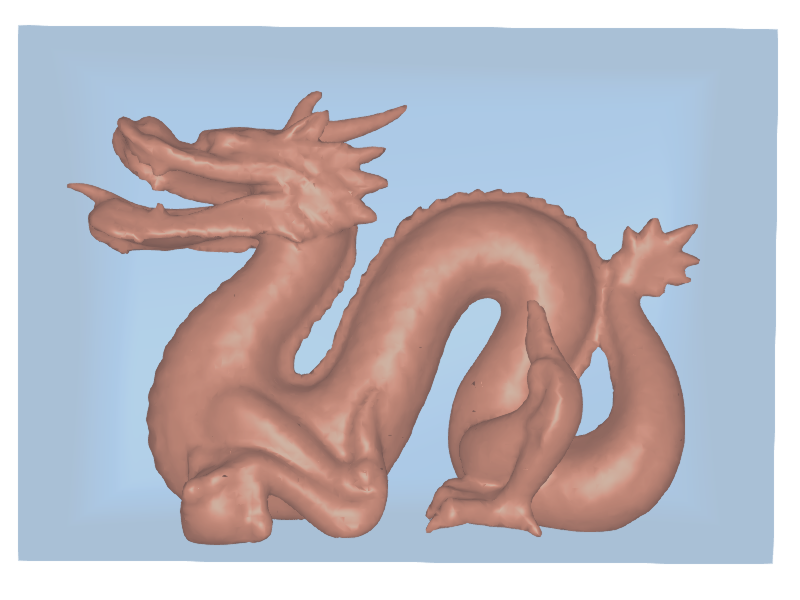
\includegraphics[width=0.5\textwidth]{skdtree_construction/tree_level_1.png}
        \caption{Επίπεδο $1$ (ρίζα)}        
    \end{subfigure}
    \begin{subfigure}{0.5\textwidth}
        \centering
        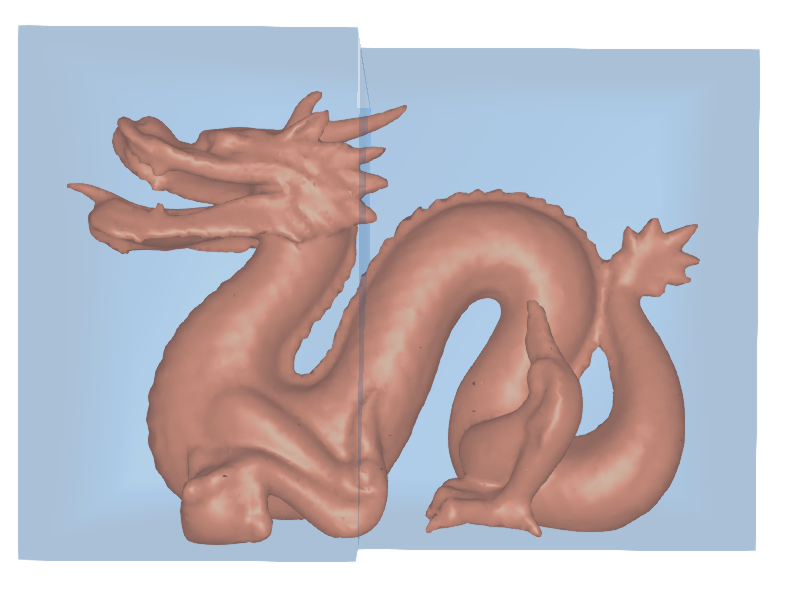
\includegraphics[width=0.5\textwidth]{skdtree_construction/tree_level_2.png}
        \caption{Επίπεδο $2$}        
    \end{subfigure}
    \begin{subfigure}{0.5\textwidth}
        \centering
        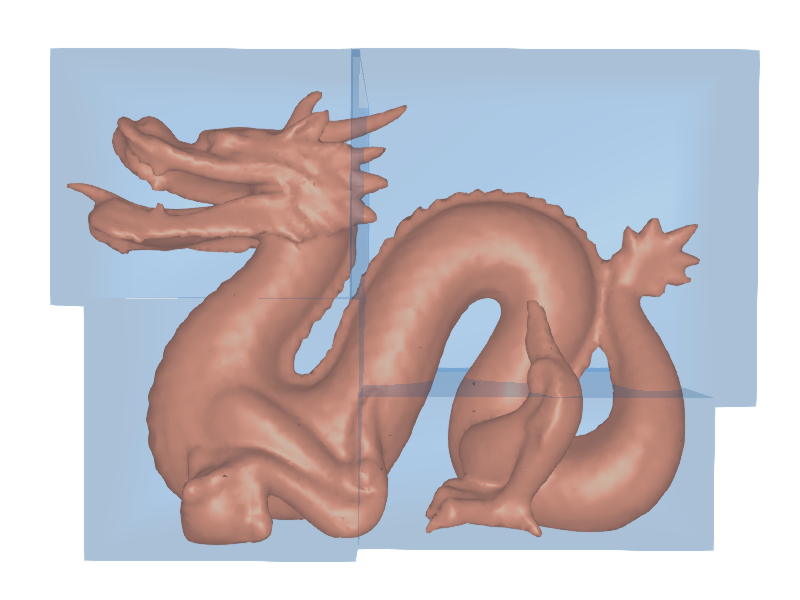
\includegraphics[width=0.5\textwidth]{skdtree_construction/tree_level_3.png}
        \caption{Επίπεδο $3$}        
    \end{subfigure}
    \begin{subfigure}{0.5\textwidth}
        \centering
        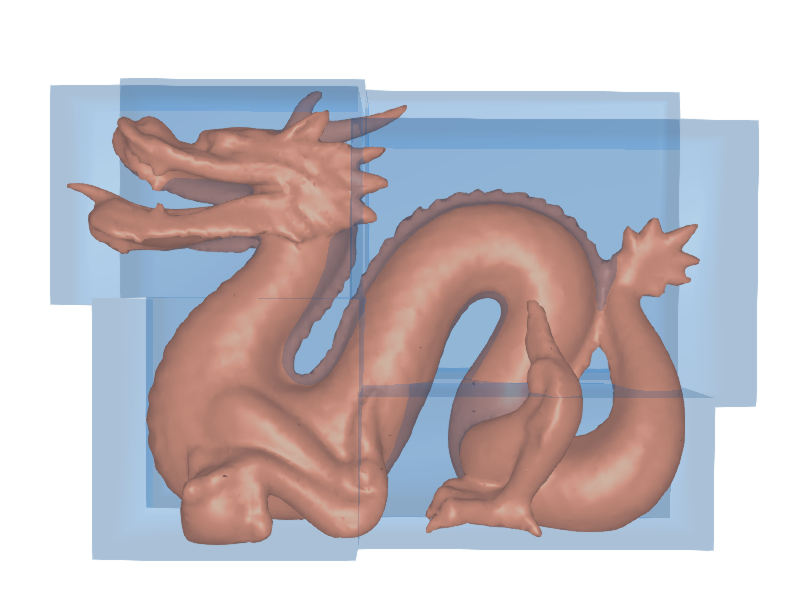
\includegraphics[width=0.5\textwidth]{skdtree_construction/tree_level_4.png}
        \caption{Επίπεδο $4$}        
    \end{subfigure}
    \begin{subfigure}{0.5\textwidth}
        \centering
        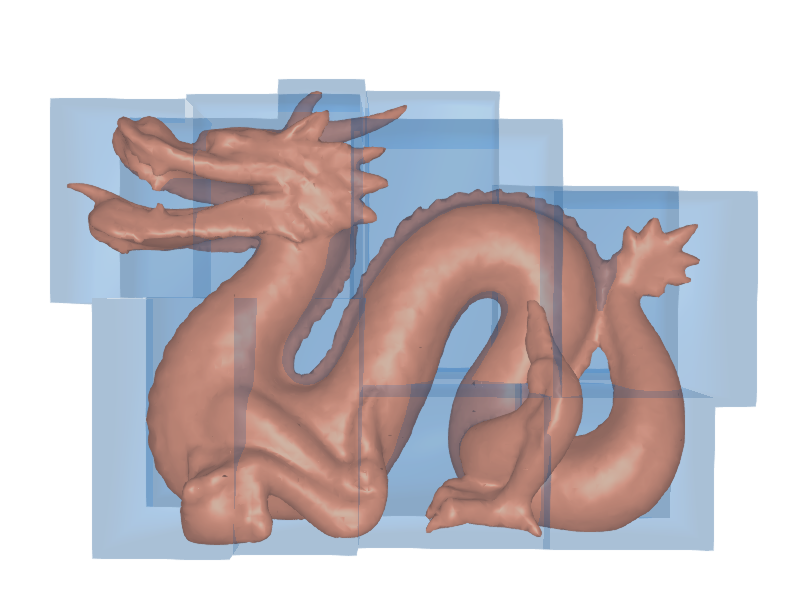
\includegraphics[width=0.5\textwidth]{skdtree_construction/tree_level_5.png}
        \caption{Επίπεδο $5$}        
    \end{subfigure}
    \begin{subfigure}{0.5\textwidth}
        \centering
        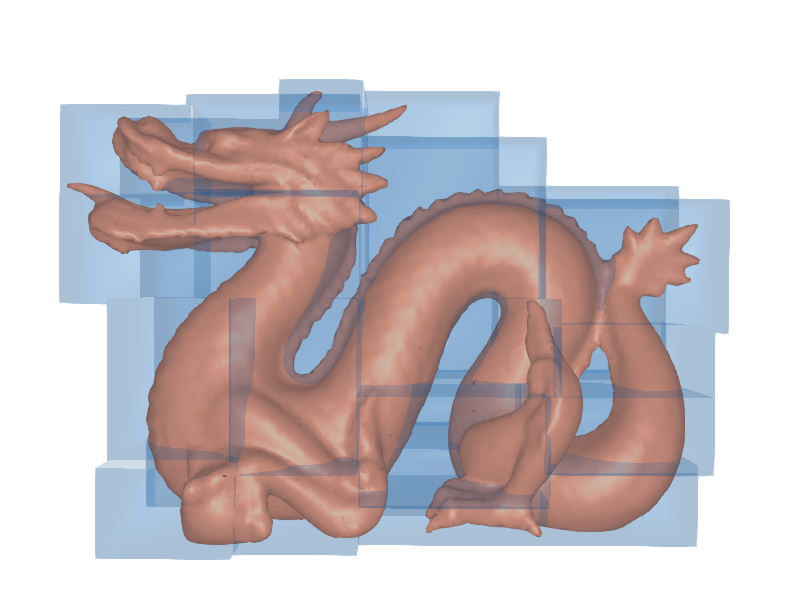
\includegraphics[width=0.5\textwidth]{skdtree_construction/tree_level_6.png}
        \caption{Επίπεδο $6$}        
    \end{subfigure}
    \begin{subfigure}{0.5\textwidth}
        \centering
        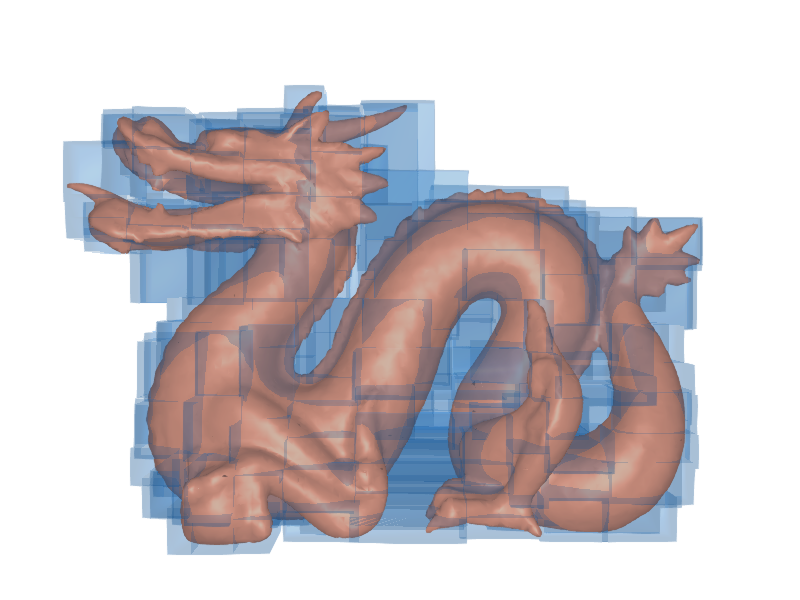
\includegraphics[width=0.5\textwidth]{skdtree_construction/tree_level_9.png}
        \caption{Επίπεδο $9$}        
    \end{subfigure}
    \begin{subfigure}{0.5\textwidth}
        \centering
        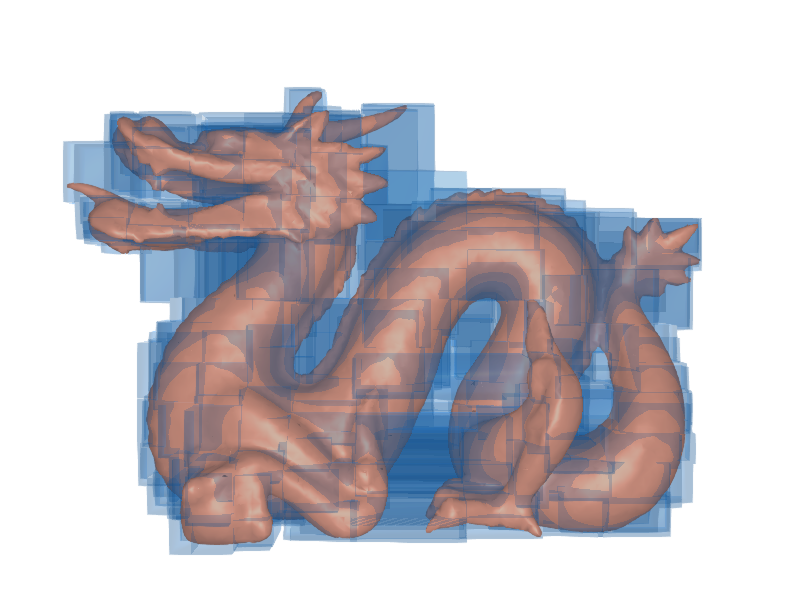
\includegraphics[width=0.5\textwidth]{skdtree_construction/tree_level_10.png}
        \caption{Επίπεδο $10$}        
    \end{subfigure}
    \begin{subfigure}{0.5\textwidth}
        \centering
        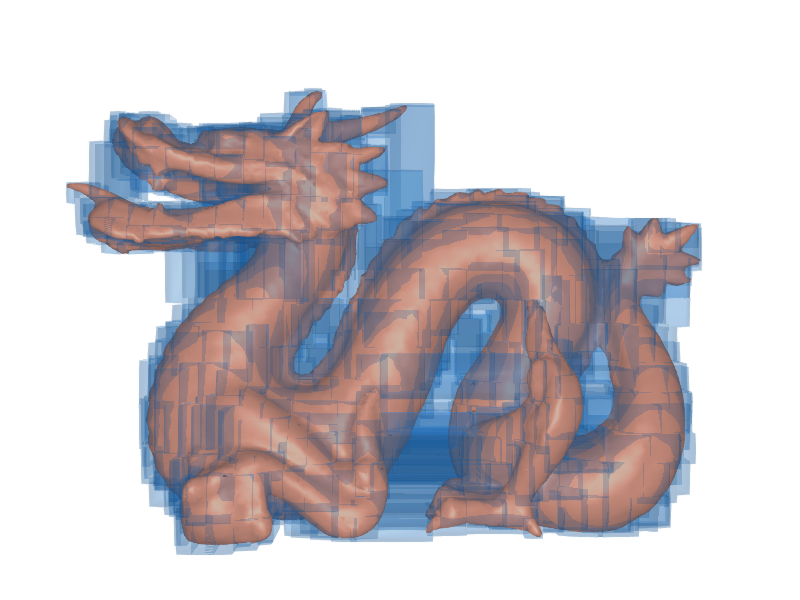
\includegraphics[width=0.5\textwidth]{skdtree_construction/tree_level_11.png}
        \caption{Επίπεδο $11$}        
    \end{subfigure}
    \begin{subfigure}{0.5\textwidth}
        \centering
        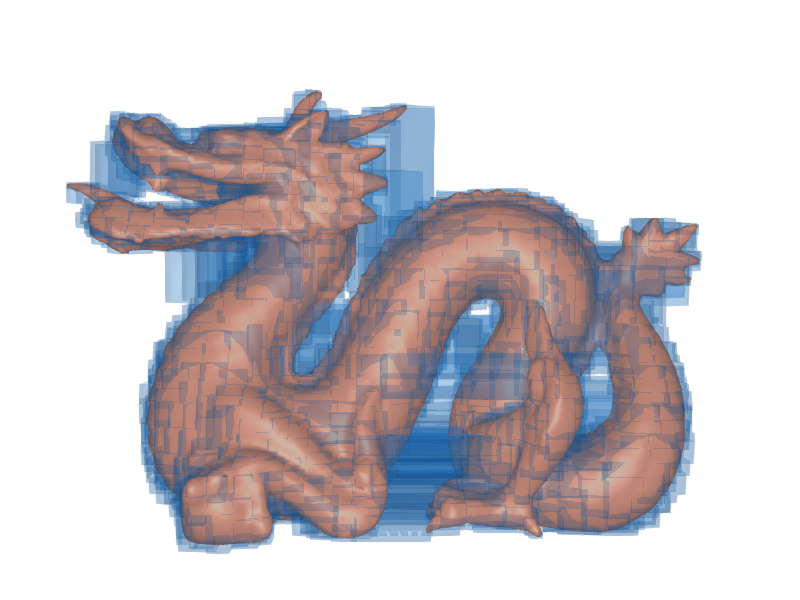
\includegraphics[width=0.5\textwidth]{skdtree_construction/tree_level_12.png}
        \caption{Επίπεδο $12$}        
    \end{subfigure}
    \begin{subfigure}{0.5\textwidth}
        \centering
        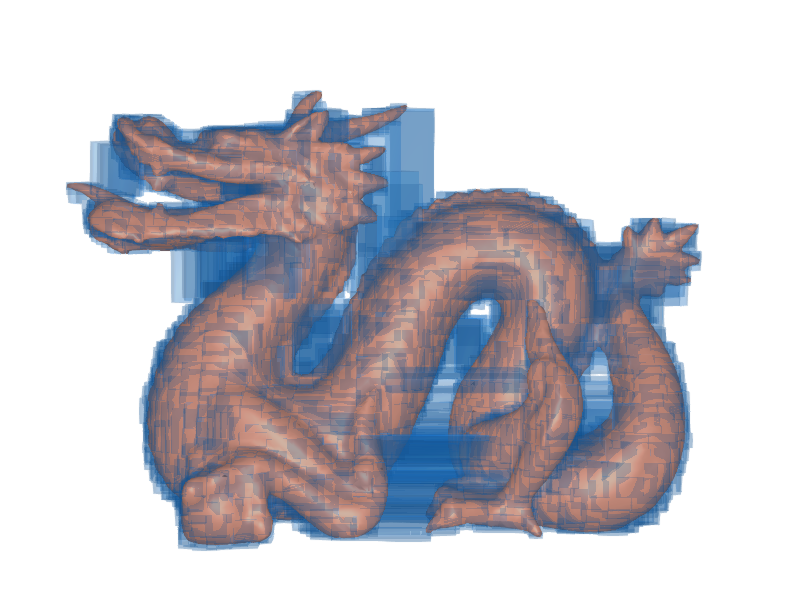
\includegraphics[width=0.5\textwidth]{skdtree_construction/tree_level_13.png}
        \caption{Επίπεδο $13$}        
    \end{subfigure}
    \begin{subfigure}{0.5\textwidth}
        \centering
        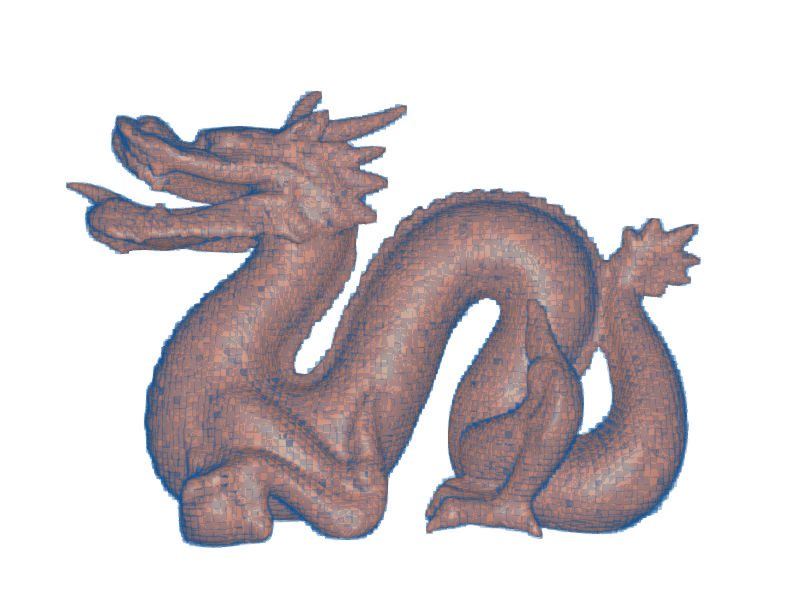
\includegraphics[width=0.5\textwidth]{skdtree_construction/tree_leaves.png}
        \caption{Φύλλα του δέντρου}        
    \end{subfigure}

    \caption[Κατασκευή \tl{sKD-Tree}]{
        Κατασκευή \tl{sKD-Tree} για το \tl{Stanford Dragon} - 
        Οι διάφορες εικόνες 
        αναπαριστούν κάποια επίπεδα του δέντρου.
        Η τελευταία εικόνα απεικονίζει τα φύλλα του 
        δέντρου. \footnote{Το \tl{sKD-Tree} είναι ένα 
        σχεδόν πλήρες δέντρο, επομένως τα φύλλα του 
        μπορούν να καταλαμβάνουν τα δύο τελευταία επίπεδα
        του δέντρου.}
    }
    \label{fig:tree_construction}
\end{figure}

\subsection{Ερωτήματα Κοντινότερου Γείτονα στο \tl{sKD-Tree}}
Δοθέντος ενός συνόλου $T$ που αποτελείται από τρίγωνα και ενός 
τυχαίου τριγώνου $q$ (\tl{\textit{query-triangle}}) αναζητούμε 
το τρίγωνο $t \in T$ που απέχει τη μικρότερη Ευκλείδεια απόσταση 
από το $q$. 
Το πρόβλημα αυτό αποτελεί γενίκευση του \tl{kNN} για χωρικά 
αντικείμενα, που στην περίπτωση μας είναι τρίγωνα που 
σχηματίζουν κάποιο πλέγμα.
Προφανώς, όπως αναφέρθηκε παραπάνω, η μεθοδολογία  
που προτείνουμε μπορεί να γενικευτεί και για άλλα στοιχεία
πέραν των τριγώνων.

Η διαδικασία διάσχισης του \tl{sKD-Tree} που προτείνουμε
για την απάντηση ερωτημάτων κοντινότερου γείτονα είναι μια 
κατευθυνόμενη αναζήτηση κατά βάθος (\tl{DFS}).
Αρχικά, επιλέγεται ένα μονοπάτι από τη ρίζα έως κάποιο φύλλο, το 
οποίο είναι η πρώτη εκτίμηση κοντινότερου γείτονα.
Για τον γείτονα αυτόν υπολογίζεται μια απόσταση.
Αυτή η απόσταση ενημερώνεται κάθε φορά που εντοπίζεται 
όλο και κοντινότερος γείτονας.
Κατά την οπισθοδρόμηση (\tl{backtracking}) η διαδικασία χρησιμοποιώντας 
την τρέχουσα εκτίμηση απόστασης κοντινότερου γείτονα απορρίπτει 
μονοπάτια του δέντρου βάση του λήμματος \ref{lemma:box_distance}.


Πιο αναλυτικά,
έστω το τυχαίο τρίγωνο $q$ του ερωτήματος.
Αρχικά κατασκευάζεται το \tl{AABB} του $q$ και ορίζεται 
η απόσταση $dist$ του κοντινότερου γείτονα (έως τώρα) να είναι 
άπειρη. 
Έπειτα καλείται η αναδρομική διαδικασία αναζήτησης.
Έστω ότι η διαδικασία επισκέπτεται
κάποιον κόμβο $v$ του δέντρου. 
Αν ο $v$ είναι εσωτερικός κόμβος, ο επόμενος κόμβος 
που θα επισκεφθεί η διαδικασία επιλέγεται να είναι 
αυτός που απέχει τη μικρότερη απόσταση από το \tl{AABB}
του $q$.
Δηλαδή, υπολογίζονται οι αποστάσεις \tl{AABB-AABB} των 
δύο παιδιών του κόμβου ως προς το \tl{AABB} του $q$ και 
επιλέγεται ο κοντινότερος.  
Αν ο κόμβος $v$ είναι φύλλο, τότε υπολογίζεται η απόσταση 
τρίγωνο-τρίγωνο και ενημερώνεται η μεταβλητή $dist$ όταν
η απόσταση που υπολογίστηκε είναι μικρότερη.
Κατά την οπισθοδρόμηση της αναδρομής, δηλαδή στη δεύτερη 
επίσκεψη του κόμβου, θα πρέπει να γίνει έλεγχος αν 
μπορεί να απορριφθεί το υποδέντρο του κόμβου που 
δεν επιλέχθηκε προηγουμένως.

Τα παραπάνω περιγράφονται στους αλγορίθμους \ref{alg:nearest_search}
και \ref{alg:nearest_search_recursive}. 
Συγκεκριμένα, για τον \ref{alg:nearest_search_recursive}:
\begin{description}
    \item[γραμμές 1-4] Είναι η περίπτωση όπου η αναζήτηση έχει 
    φτάσει σε φύλλο του δέντρου, οπότε γίνεται έλεγχος απόστασης 
    του $q$ από το τρίγωνο του φύλλου.
    \item[γραμμές 5-6] Γίνεται υπολογισμός της απόστασης του 
    \tl{AABB} του $q$ με τα \tl{AABB} των παιδιών του κόμβου. 
    Αυτές οι αποστάσεις χρησιμοποιούνται για να καθοδηγήσουν 
    την αναζήτηση.
    \item[γραμμές 7,15] Γίνεται καθοδήγηση της σειράς με την 
    οποία θα γίνει η αναζήτηση.
    \item[γραμμές 8-13] Πρώτα γίνεται αναζήτηση στο αριστερό 
    παιδί και έπειτα στο δεξί.
    \item[γραμμές 16-21] Πρώτα γίνεται αναζήτηση στο δεξί 
    παιδί και έπειτα στο αριστερό.
    \item[γραμμές 11,19] Έλεγχος για το αν είναι απαραίτητη 
    η επίσκεψη στο παιδί που δεν επιλέχθηκε προηγουμένως.
    \item[γραμμές 8,16] Πρόωρο τερματισμό της 
    αναζήτησης (\tl{early exit}). 
    Αυτό είναι χρήσιμο όταν ένας κόμβος δεν μπορεί να 
    απορριφθεί κατά την αναζήτηση, όμως μπορούν να 
    απορριφθούν τα παιδιά του.
    Έτσι η αναζήτηση δε χρειάζεται να φτάσει μέχρι 
    το φύλλο του υποδέντρου.
\end{description}

\selectlanguage{english}
\IncMargin{1.5em}
\begin{algorithm}[h]
    \caption[Υπολογισμός Απόστασης Κοντινότερου Γείτονα]{
        \tg{Υπολογισμός Απόστασης Κοντινότερου Γείτονα}
        }
    \label{alg:nearest_search}
    \DontPrintSemicolon
    \KwIn{An sKD-Tree $tree$, a query-triangle $q$, a search radius $r$ (optional)}
    \KwOut{The distance of the nearest neighbor}
    \SetKwFunction{nearestsearch}{nearest\_search}
    \SetKwFunction{nearestsearchrecur}{nearest\_search\_recursive}
    \Indm\nonl\nearestsearch($tree$, $q$)\\
    \Indp
        precalculate the AABB of $q$ \;
        $distance \gets \infty$ \;
        \nearestsearchrecur($tree.root$, $q$, $distance$)\;
        \Return{$distance$}

\end{algorithm}
\DecMargin{1.5em}
\selectlanguage{greek}

\selectlanguage{english}
\IncMargin{1.5em}
\begin{algorithm}[h]
    \caption[Αναδρομικός Υπολογισμός Απόστασης Κοντινότερου Γείτονα]{
        \tg{Αναδρομικός Υπολογισμός Απόστασης Κοντινότερου Γείτονα}
    }
    \label{alg:nearest_search_recursive}
    \DontPrintSemicolon
    \KwIn{An sKD-Tree node $v$, a query-triangle $q$, NN distance so far $distance$}
    \KwOut{Changes $distance$ to be the distance of the nearest neighbor}
    \Indm\nonl\nearestsearchrecur($v$, $q$, $distance$)\\
    \Indp
        \If{$v$ is leaf}{
            $distance \gets \min(distance, \dist(q, v.triangle))$ \;
            \Return{}
        }

        $aabb\_dist\_l \gets \aabbdist(\aabb(q), v.left.aabb)$\;
        $aabb\_dist\_r \gets \aabbdist(\aabb(q), v.right.aabb)$\;
        \If{$distance_{left} < distance_{right}$}{
            \If{$distance_{left} < distance$}{
                \nearestsearchrecur($v.left$, $q$, $distance$)
            }
            \If{$distance_{right} < distance$}{
                \nearestsearchrecur($v.right$, $q$, $distance$)
            }
        }
        \Else{
            \If{$distance_{right} < distance$}{
                \nearestsearchrecur($v.right$, $q$, $distance$)
            }
            \If{$distance_{left} < distance$}{
                \nearestsearchrecur($v.left$, $q$, $distance$)
            }
        }
        \Return{}

\end{algorithm}
\DecMargin{1.5em}
\selectlanguage{greek}

Σημειώνουμε ότι δεν είναι εφικτό να υπολογίσουμε την πολυπλοκότητα 
του αλγορίθμου αναζήτησης ούτε να εγγυηθούμε καλή επίδοση 
χειρότερης περίπτωσης. 
Αυτό οφείλεται στο ότι κατά την αναζήτηση μπορεί να γίνει 
επίσκεψη και στα δύο υποδέντρα ενός κόμβου (ή μέρος τους).

\section{Αλγόριθμοι που χρησιμοποιούν τη δομή \tl{sKD-Tree}}

\section{Βελτιστοποίηση των Αλγορίθμων για Πραγματικά Συστήματα Υπολογιστών}
\subsection{Παραλληλοποίηση με χρήση Πολλαπλών Νημάτων \tl{(Multi-threading)}}
\subsection{Χρήση Κουβάδων στα Φύλλα του \tl{sKD-Tree (Buckets)}}